\titlespacing*{\part}{0pt}{-20pt}{30pt} % to fix table and plot together on the first page (SEE RESTORE AT BOTTOM)
\titlespacing*{\chapter}{0pt}{-10pt}{30pt}

\part{Supervised Learning} % DIFF: top-level "part" is Supervised Learning (while "Linear Regression" is a chapter)
\label{part:supervised_learning}

\marginnote{From CS229 Fall 2020, Tengyu Ma, Andrew Ng \& Chris R\'e, Stanford University.}


Let's start by talking about a few examples of supervised learning problems.
Suppose we have a dataset giving the living areas and prices of 47 houses
from Portland, Oregon:

\begin{table}[!h]
  \centering
  \caption{
    \label{tab:houses} Housing prices in Portland, OR.
  }
  \begin{tabular}{cc}
    \toprule
    Living area (feet$^2$) & Price (1000\$s) \\
    \midrule
    2104 & 400 \\
    1600 & 330 \\
    2400 & 369 \\
    1416 & 232 \\
    3000 & 540 \\
    $\vdots$ & $\vdots$ \\
    \bottomrule
  \end{tabular}
\end{table}

\phantom{} % extra newline space

We can plot this data:
\begin{figure}
    \caption{
        \label{fig:houses} Housing prices in Portland, OR.
    }
    \begin{jlcode}
    p = let
        data = CSV.read("..\\data\\portland-houses.csv", DataFrame; header=["area", "bedrooms", "price"])
        X = data[:area]
        Y = data[:price] ./ 1000

        Axis(Plots.Scatter(X, Y, style="mark=x"), title="housing prices", xlabel="square feet", ylabel="price (in \\\$1000)", xmax=5000, ymax=800)
    end
    plot(p)
    \end{jlcode}
    \begin{center}
        \plot{fig/portland_houses}
    \end{center}
\end{figure}


Given data like this, how can we learn to predict the prices of other houses
in Portland, as a function of the size of their living areas?

To establish notation for future use, we'll use $x^{(i)}$ to denote the ``input''
variables (living area in this example), also called input \textbf{features}, and $y^{(i)}$
to denote the ``output'' or \textbf{target} variable that we are trying to predict
(price). A pair $(x^{(i)}, y^{(i)})$ is called a \textbf{training example}, and the dataset
that we'll be using to learn---a list of $n$ training examples $\{(x^{(i)}, y^{(i)} );\; i =
1,\ldots,n\}$---is called a \textbf{training set}. Note that the superscript ``$(i)$'' in the
notation is simply an index into the training set, and has nothing to do with
exponentiation. We will also use $\cal X$ denote the space of input values, and $\cal Y$
the space of output values. In this example, $\cal X = \cal Y = \bb R$.

To describe the supervised learning problem slightly more formally, our
goal is, given a training set, to learn a function $h: \cal X \mapsto \cal Y$ so that $h(x)$ is a
``good'' predictor for the corresponding value of $y$. For historical reasons, this
function $h$ is called a \textbf{hypothesis}. Seen pictorially, the process is therefore
like this:

\begin{figure}
\begin{center}
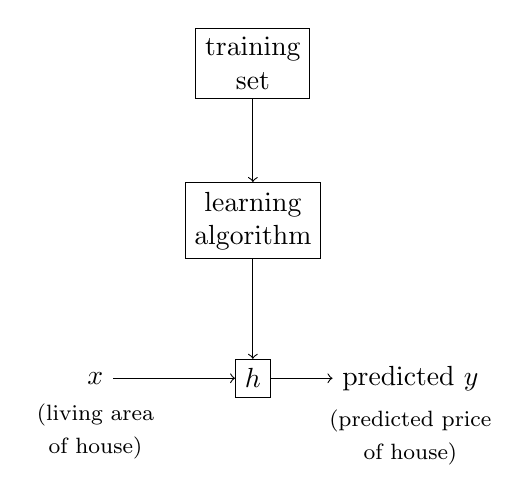
\begin{tikzpicture}[node distance=2cm, auto]
    \node [rectangle, align=center, draw] (training) {training\\set};
    \node [rectangle, align=center, draw, below of=training] (learning) {learning\\algorithm};
    \node [rectangle, align=center, draw, below of=learning] (h) {$h$};
    \node [left of=h, label={[align=center]below:\footnotesize (living area\\\footnotesize of house)}] (x) {$x$};
    \node [right of=h, label={[align=center]below:\footnotesize (predicted price\\\footnotesize of house)}] (y) {predicted $y$};

    \path [->, draw] (training) -- (learning);
    \path [->, draw] (learning) -- (h);
    \path [->, draw] (x) -- (h);
    \path [->, draw] (h) -- (y);
\end{tikzpicture}
\caption{\label{fig:hypothesis} Hypothesis diagram.}
\end{center}
\end{figure}

% TODO: get Francis Galton citation.
When the target variable that we're trying to predict is continuous, such
as in our housing example, we call the learning problem a \textbf{regression}\footnote{The term \textit{regression} was originally coined due to ``regressing'' to the mean (Francis Galton, 1886).} problem. % DIFF: regression term explanation.
When $y$ can take on only a small number of discrete values (such as
if, given the living area, we wanted to predict if a dwelling is a house or an
apartment, say), we call it a \textbf{classification} problem.


\chapter{Linear Regression}
\label{cha:linear_regression}

To make our housing example more interesting, let's consider a slightly richer
dataset in which we also know the number of bedrooms in each house:


\begin{table}[!h]
  \centering
  \caption{
    \label{tab:bedrooms} Housing prices with bedrooms in Portland, OR.
  }
  \begin{tabular}{ccc}
    \toprule
    Living area (feet$^2$) & \texttt{\#} Bedrooms & Price (1000\$s) \\
    \midrule
    2104 & 3 & 400 \\
    1600 & 3 & 330 \\
    2400 & 3 & 369 \\
    1416 & 2 & 232 \\
    3000 & 4 & 540 \\
    $\vdots$ & $\vdots$ & $\vdots$ \\
    \bottomrule
  \end{tabular}
\end{table}

Here, the $x$'s are two-dimensional vectors in $\bb R^2$. For instance, $x^{(i)}_1$
is the living area of the $i$-th house in the training set, and $x^{(i)}_2$
is its number of bedrooms.\footnote{In general, when designing a learning problem, it will be up to % DIFF: turned this parenthetical into a footnote
you to decide what features to choose, so if you are out in Portland gathering
housing data, you might also decide to include other features such as whether
each house has a fireplace, the number of bathrooms, and so on. We'll say
more about feature selection later, but for now let's take the features as
given.}

To perform supervised learning, we must decide how we're going to represent
functions/hypotheses $h$ in a computer. As an initial choice, let's say
we decide to approximate $y$ as a linear function of $x$:

\begin{equation}
    h_\theta(x) = \theta_0 + \theta_1 x_1 + \theta_2 x_2
\end{equation}

Here, the $\theta_i$'s are the \textbf{parameters} (also called \textbf{weights}) parameterizing the
space of linear functions mapping from $\cal X$ to $\cal Y$. When there is no risk of
confusion, we will drop the $\theta$ subscript in $h_\theta(x)$, and write it more simply as
$h(x)$. To simplify our notation, we also introduce the convention of letting
$x_0 = 1$ (this is the intercept term), so that

\begin{equation}
    h(x) = \sum_{i=0}^d \theta_i x_i = \theta^\top x\text{,} % DIFF: \top instead of ^T
\end{equation}

where on the right-hand side above we are viewing $\theta$ and $x$ both as vectors,
and here $d$ is the number of input variables (not counting $x_0$).

Now, given a training set, how do we pick, or learn, the parameters $\theta$?
One reasonable method seems to be to make $h(x)$ close to $y$, at least for
the training examples we have. To formalize this, we will define a function
that measures, for each value of the $\theta$'s, how close the $h(x^{(i)})$'s are to the
corresponding $y^{(i)}$'s. We define the \textbf{cost function}:

\begin{equation}
    J(\theta) = \frac 1 2 \sum_{i=1}^n \left( h_\theta(x^{(i)}) - y^{(i)} \right)^2\text{.}
\end{equation}

If you've seen linear regression before, you may recognize this as the familiar
least-squares cost function that gives rise to the \textbf{ordinary least squares}
regression model. Whether or not you have seen it previously, let's keep
going, and we'll eventually show this to be a special case of a much broader
family of algorithms.


\section{Least mean squares (LMS) algorithm} % DIFF: spelled out LMS

We want to choose $\theta$ so as to minimize $J(\theta)$. To do so, let's use a search
algorithm that starts with some ``initial guess'' for $\theta$, and that repeatedly
changes $\theta$ to make $J(\theta)$ smaller, until hopefully we converge to a value of
$\theta$ that minimizes $J(\theta)$. Specifically, let's consider the \textbf{gradient descent}
algorithm, which starts with some initial $\theta$, and repeatedly performs the
update:\footnote{This update is simultaneously performed for all values of $j = 0,\ldots,d$.} % DIFF: made parenthetical a footnote
%
\begin{equation}
    \theta_j \leftarrow \theta_j - \alpha \frac{\partial}{\partial \theta_j} J(\theta) % DIFF: Changed := to \leftarrow for update
\end{equation}
%
Here, $\alpha$ is called the \textbf{learning rate}. This is a very natural algorithm that
repeatedly takes a step in the direction of steepest decrease of $J$.

In order to implement this algorithm, we have to work out what is the
partial derivative term on the right hand side. Let's first work it out for the
case of if we have only one training example $(x,y)$, so that we can neglect
the sum in the definition of $J$. We have:

\begin{align*}
    \frac{\partial}{\partial \theta_j} J(\theta) &= \frac{\partial}{\partial \theta_j} \frac 1 2 \left( h_\theta(x) - y \right)^2\\
    &= 2 \cdot \frac 1 2 (h_\theta(x) - y) \cdot \frac{\partial}{\partial \theta_j} (h_\theta(x) - y) \\
    &= (h_\theta(x) - y) \cdot \frac{\partial}{\partial \theta_j} \left( \sum_{i=0}^d \theta_i x_i - y \right) \\
    &= (h_\theta(x) - y) x_j
\end{align*}

For a single training example, this gives the update rule:\footnote{We use the notation ``$a \leftarrow b$'' to denote an operation (in a computer program) in
which we set the value of a variable $a$ to be equal to the value of $b$ (something $:=$ is used). In other words, this
operation overwrites $a$ with the value of $b$. In contrast, we will write ``$a = b$'' when we are
asserting a statement of fact, that the value of $a$ is equal to the value of $b$.}

\begin{equation}
    \theta_j \leftarrow \theta_j + \alpha \left( y^{(i)} - h_\theta(x^{(i)}) \right) x^{(i)}_j \text{.} % DIFF: \leftarrow (:=)
\end{equation}

The rule is called the \textbf{LMS} update rule (LMS stands for ``least mean squares''),
and is also known as the \textbf{Widrow-Hoff} learning rule. This rule has several
properties that seem natural and intuitive. For instance, the magnitude of
the update is proportional to the \textbf{error} term $(y^{(i)} - h_\theta(x^{(i)}))$; thus, for
instance, if we are encountering a training example on which our prediction
nearly matches the actual value of $y^{(i)}$, then we find that there is little need
to change the parameters; in contrast, a larger change to the parameters will
be made if our prediction $h_\theta(x^{(i)})$ has a large error (i.e., if it is very far from
$y^{(i)}$).

We've derived the LMS rule for when there was only a single training % DIFF: we'd to we've
example. There are two ways to modify this method for a training set of
more than one example. The first is replace it with the following algorithm:

% DIFF: cleaned up this algorithm block (broke out the for loop).
\begin{algorithm}[ht]
    \caption{Gradient descent.}
    \label{alg:gd}
    \begin{algorithmic}
    \Repeat
        \For{every $j$}
            \State $\theta_j \leftarrow \theta_j + \alpha \displaystyle\sum\limits_{i=1}^n \left( y^{(i)} - h_\theta(x^{(i)}) \right) x^{(i)}_j$ %, \quad (for every $j$)
        \EndFor
    \Until{convergence}
    \end{algorithmic}
\end{algorithm}

By grouping the updates of the coordinates into an update of the vector
$\theta$, we can rewrite update \cref{alg:gd} in a slightly more succinct way:

\begin{algorithm}[ht]
    \caption{Gradient descent vectorized.}
    \label{alg:gd_vector}
    \begin{algorithmic}
    \Repeat
        \State $\theta \leftarrow \theta + \alpha \displaystyle\sum\limits_{i=1}^n \left( y^{(i)} - h_\theta(x^{(i)}) \right) x^{(i)}$
    \Until{convergence}
    \end{algorithmic}
\end{algorithm}

The reader can easily verify that the quantity in the summation in the
update rule above is just $\partial J(\theta) / \partial \theta_j$ (for the original definition of $J$).
So, this is simply gradient descent on the original cost function $J$. This method looks
at every example in the entire training set on every step, and is called \textbf{batch gradient descent}.
Note that, while gradient descent can be susceptible
to local minima in general, the optimization problem we have posed here
for linear regression has only one global, and no other local, optima; thus
gradient descent always converges (assuming the learning rate $\alpha$ is not too
large) to the global minimum. Indeed, $J$ is a convex quadratic function.


% TODO: Julia code (gradient descent—see alg4ai and "gradient_descent.jl")


\begin{example}
    \caption{\label{ex:gd} Gradient descent on a quadratic function.}

    Here is an example of gradient descent as it is run to minimize a quadratic
    function.

    \begin{jlcode}
    p = let
        @vars x, y
        f = x^2/2 + y^2
        plot_gradient_descent(f, initial=[48, 30], path_length=40)
    end
    plot(p)
    \end{jlcode}
    \begin{center}
        \plot{fig/gradient_descent}
    \end{center}

    The ellipses shown above are the contours of a quadratic function. Also
    shown is the trajectory taken by gradient descent, which was initialized at
    (48,30). The arrows in the figure (joined by straight lines) mark the successive % DIFF: changed $x$'s to arrows.
    values of $\theta$ that gradient descent went through.
\end{example}


\begin{example}
    % TODO: Generate \theta's directly from `linear_regression' (see plots-notebook.jl)
    When we run batch gradient descent to fit $\theta$ on our previous dataset,
    to learn to predict housing price as a function of living area. We obtain: % DIFF: split into two sentences.
    \begin{align*} % DIFF: put these in their own newlined equation block AND added \tag annotations.
        \theta_0 &= 71.27 \tag{intercept}\\
        \theta_1 &= 0.1345 \tag{slope}
    \end{align*}
    If we plot $h_\theta (x)$ as a function of $x$ (area), along
    with the training data, we obtain the following figure:

    \caption{
        % TODO I actually use linear regression here and not batch gradient descent.
        \label{ex:linear_regression} Best fit line using batch gradient descent on Portland, Oregon housing prices.
    }
    \begin{jlcode}
    p = let
        data = CSV.read("..\\data\\portland-houses.csv", DataFrame; header=["area", "bedrooms", "price"])
        X = data[:area]
        Y = data[:price] ./ 1000

        h = linear_regression(X, Y)

        p_data = Plots.Scatter(X, Y, style="mark=x")
        xn = (minimum(X) - 500):5000 # (maximum(X) + 500)

        p_fit = Plots.Linear(xn, h.(xn), style="blue, no marks")

        Axis([p_data, p_fit], title="housing prices", xlabel="square feet", ylabel="price (in \\\$1000)", xmin=first(xn), xmax=last(xn), ymax=800)
    end
    plot(p)
    \end{jlcode}
    \begin{center}
        \plot{fig/linear_regression}
    \end{center}

    % TODO: Generate \theta's directly from `linear_regression'
    If the number of bedrooms were included as one of the input features as well,
    we get $\theta_0 = 89.60, \theta_1 = 0.1392, \theta_2 = -8.738$.
\end{example}


% TODO: obtain these results with batch gradient descent.
The results in \cref{ex:linear_regression} were obtained with batch gradient descent. There is
an alternative to batch gradient descent that also works very well. Consider
the following algorithm:

% DIFF: Cleaned up the algorithm.
\begin{algorithm}[ht]
    \caption{Stochastic gradient descent.}
    \label{alg:sgd}
    \begin{algorithmic}
    \Repeat
        \For{$i = 1$ to $n$}
            \For{every $j$}
                \State $\theta_j \leftarrow \theta_j + \alpha \displaystyle\sum\limits_{i=1}^n \left( y^{(i)} - h_\theta(x^{(i)}) \right) x^{(i)}_j$ %, \quad (for every $j$)
            \EndFor
        \EndFor
    \Until{convergence}
    \end{algorithmic}
\end{algorithm}

By grouping the updates of the coordinates into an update of the vector
$\theta$, we can rewrite update in \cref{alg:sgd} in a slightly more succinct way:

\begin{equation}
    \theta \leftarrow \theta + \alpha \left( y^{(i)} - h_\theta^{(i)} \right) x^{(i)}
\end{equation}

In this algorithm, we repeatedly run through the training set, and each
time we encounter a training example, we update the parameters according
to the gradient of the error with respect to that single training example only.
This algorithm is called \textbf{stochastic gradient descent} (also \textbf{incremental
gradient descent}). Whereas batch gradient descent has to scan through
the entire training set before taking a single step---a costly operation if $n$ is
large---stochastic gradient descent can start making progress right away, and
continues to make progress with each example it looks at. Often, stochastic
gradient descent gets $\theta$ ``close'' to the minimum much faster than batch gradient
descent.\footnote{Note, however, that it may never ``converge'' to the minimum,
and the parameters $\theta$ will keep oscillating around the minimum of $J(\theta)$; but
in practice most of the values near the minimum will be reasonably good
approximations to the true minimum. By slowly letting the learning rate $\alpha$ decrease to
zero as the algorithm runs, it is also possible to ensure that the parameters will converge to
the global minimum rather than merely oscillate around the minimum.} % DIFF: combined parenthetical and footnote.
For these reasons, particularly when the training set is large,
stochastic gradient descent is often preferred over batch gradient descent.


\section{The normal equations}
\label{sec:the_normal_equations}

Gradient descent gives one way of minimizing $J$. Let's discuss a second way
of doing so, this time performing the minimization explicitly and without
resorting to an iterative algorithm. In this method, we will minimize $J$ by
explicitly taking its derivatives with respect to the $\theta_j$'s, and setting them to
zero. To enable us to do this without having to write reams of algebra and
pages full of matrices of derivatives, let's introduce some notation for doing
calculus with matrices.

\subsection{Matrix derivatives}
For a function $f : \bb R^{n \times d} \mapsto \bb R$ mapping from $n$-by-$d$ matrices to the real
numbers, we define the derivative of $f$ with respect to $A$ to be:

\begin{equation}
    \nabla_A f(A) = \begin{bmatrix}
        \frac{\partial f}{\partial A_{11}} & \cdots & \frac{\partial f}{\partial A_{1d}} \\
        \vdots & \ddots & \vdots \\
        \frac{\partial f}{\partial A_{n1}} & \cdots & \frac{\partial f}{\partial A_{nd}} \\
    \end{bmatrix}
\end{equation}

Thus, the gradient $\nabla_A f(A)$ is itself an $n$-by-$d$ matrix, whose $(i,j)$-element is
$\partial f / \partial A_{ij}$.

\begin{example}
    \caption{\label{ex:matrix_derivative}Matrix derivative.}

    For example, suppose $A =
    \begin{bmatrix}
        A_{11} & A_{12} \\
        A_{21} & A_{22}
    \end{bmatrix}$
    is a 2-by-2 matrix, and the function $f : \bb R^{2\times2} \mapsto \bb R$ is given by
    \begin{equation*}
        f(A) = \frac 3 2 A_{11} + 5 A_{12}^2 + A_{21}A_{22}\text{.}
    \end{equation*}
    Here, $A_{ij}$ denotes the $(i,j)$ entry of the matrix $A$. We then have:
    \begin{equation*}
        \nabla_A f(A) =
        \begin{bmatrix}
            \frac 3 2 & 10 A_{12} \\
            A_{22} & A_{21}
        \end{bmatrix}
    \end{equation*}
\end{example}


\subsection{Least squares revisited}

% TODO: \vec \theta ???? (CHANGE THROUGHOUT)

Armed with the tools of matrix derivatives, let us now proceed to find in
closed-form the value of $\theta$ that minimizes $J(\theta)$. We begin by re-writing $J$ in
matrix-vector notation. % DIFF: changed from "matrix-vectorial" to "matrix-vector"

% DIFF: bold-faced matrix $\mat X$
Given a training set, define the \textbf{design matrix} $\mat X$ to be the $n$-by-$d$ matrix
(actually $n$-by-$(d + 1)$, if we include the intercept term) that contains the % DIFF: added (...) around d+1
training examples' input values in its rows:

% DIFF: \top not ^T, bold-faced matrix (from here on out.)
\begin{equation}
    \mat X = \begin{bmatrix}
        \text{--- } (x^{(1)})^\top \text{ ---} \\
        \text{--- } (x^{(2)})^\top \text{ ---} \\
        \vdots \\
        \text{--- } (x^{(n)})^\top \text{ ---}
    \end{bmatrix}
\end{equation}
% DIFF: bold-face vector notation (not above-arrow, from here on out.)
Also, let $\vec y$ be the $n$-dimensional vector containing all the target values from
the training set:
\begin{equation}
    \vec y = \begin{bmatrix}
        y^{(1)} \\
        y^{(2)} \\
        \vdots \\
        y^{(n)}
    \end{bmatrix}
\end{equation}
Now, since $h_\theta(x^{(i)}) = (x^{(i)})^\top \theta$, we can easily verify that
\begin{align*}
    \mat X \theta - \vec y &= \begin{bmatrix}
        (x^{(1)})^\top \theta \\
        \vdots \\
        (x^{(n)})^\top \theta
    \end{bmatrix}
    -
    \begin{bmatrix}
        y^{(1)} \\    
        \vdots \\
        y^{(n)}    
    \end{bmatrix}\\
    &= \begin{bmatrix}
        h_\theta(x^{(1)}) - y^{(1)} \\
        \vdots \\
        h_\theta(x^{(n)}) - y^{(n)}
    \end{bmatrix}\text{.}
\end{align*}
Thus, using the fact that for a vector $z$, we have that $z^\top z = \sum_i z_i^2$:
\begin{align*}
    \frac 1 2 (\mat X \theta - \vec y)^\top (\mat X \theta - \vec y) &= \frac 1 2 \sum_{i=1}^n \left( h_\theta(x^{(i)}) - y^{(i)} \right)^2 \\
    &= J(\theta)
\end{align*}
Finally, to minimize $J$, let's find its derivative with respect to $\theta$. Hence:
\begin{align*}
    \nabla_\theta J(\theta) &= \nabla_\theta \frac 1 2 (\mat X \theta - \vec y)^\top (\mat X \theta - \vec y) \\
                            &= \frac 1 2 \nabla_\theta \left( (\mat X \theta)^\top \mat X \theta - (\mat X \theta)^\top \vec y - \vec y^\top (\mat X \theta) + \vec y^\top \vec y \right) \\
                            &= \frac 1 2 \nabla_\theta \left( \theta^\top (\mat X^\top \mat X) \theta - \vec y^\top (\mat X \theta) - \vec y^\top (\mat X \theta) \right) \tag{$a^\top b = b^\top a$} \\
                            &= \frac 1 2 \nabla_\theta \left( \theta^\top (\mat X^\top \mat X) \theta - 2 (\mat X^\top \vec y)^\top \theta \right) \\
                            &= \frac 1 2 \left( 2\mat X^\top \mat X \theta - 2 \mat X^\top \vec y \right) \tag{$\nabla_x b^\top x = b$ and $\nabla_x x^\top A x = 2 A x$ for sym. $A$} \\
                            &= \mat X^\top \mat X \theta - \mat X^\top \vec y
\end{align*}
% DIFF: Moved "third step" and "fifth step" explanations to \tags
To minimize $J$, we set its derivatives to zero, and obtain the \textbf{normal equations}:
\begin{equation}
    \mat X^\top \mat X \theta = \mat X^\top \vec y
\end{equation}
Thus, the value of $\theta$ that minimizes $J(\theta)$ is given in closed form by the equation:
\footnote{Note that in the this step, we are implicitly assuming that $\mat X^\top \mat X$ is an invertible
matrix. This can be checked before calculating the inverse. If either the number of
linearly independent examples is fewer than the number of features, or if the features
are not linearly independent, then $\mat X^\top \mat X$ will not be invertible. Even in such cases, it is
possible to ``fix'' the situation with additional techniques, which we skip here for the sake of simplicty.}
\begin{equation}
    \theta = (\mat X^\top \mat X)^{-1} \mat X^\top \vec y
\end{equation}


\section{Probabilistic interpretation}
When faced with a regression problem, why might linear regression, and
specifically why might the least-squares cost function $J$, be a reasonable
choice? In this section, we will give a set of probabilistic assumptions, under
which least-squares regression is derived as a very natural algorithm.

Let us assume that the target variables and the inputs are related via the
equation
\begin{equation}
    y^{(i)} = \theta^\top x^{(i)} + \epsilon^{(i)}\text{,}
\end{equation}
where $\epsilon^{(i)}$ is an error term that captures either unmodeled effects (such as
if there are some features very pertinent to predicting housing price, but
that we'd left out of the regression), or random noise. Let us further assume
that the $\epsilon^{(i)}$ are distributed IID (independently and identically distributed)
according to a Gaussian distribution (also called a Normal distribution) with
mean zero and some variance $\sigma^2$. We can write this assumption as % DIFF: removed quotes
$\epsilon^{(i)} \sim \cal N(0, \sigma^2)$, i.e. the density of $\epsilon^{(i)}$ is given by
\begin{equation}
    p(\epsilon^{(i)}) = \frac{1}{\sqrt{2\pi}\sigma} \exp \left( - \frac{(\epsilon^{(i)})^2}{2\sigma^2} \right)\text{.}
\end{equation}
This implies that
\begin{equation}
    p(y^{(i)} \mid x^{(i)}; \theta) = \frac{1}{\sqrt{2\pi}\sigma} \exp \left( - \frac{(y^{(i)} - \theta^\top x^{(i)})^2}{2\sigma^2} \right)\text{.}
\end{equation}
The notation ``$p(y^{(i)} \mid x^{(i)}; \theta)$'' indicates that this is the distribution of $y^{(i)}$
given $x^{(i)}$ and parameterized by $\theta$. Note that we should not condition on $\theta$
(i.e. ``$p(y^{(i)} \mid x^{(i)}, \theta)$''), since $\theta$ is not a random variable. We can also write the
distribution of $y^{(i)}$ as $(y^{(i)} \mid x^{(i)}; \theta) \sim \cal N(\theta^\top x^{(i)}, \sigma^2)$. % DIFF: added parens

Given $\mat X$ (the design matrix, which contains all the $x^{(i)}$'s) and $\theta$, what
is the distribution of the $y^{(i)}$'s? The probability of the data is given by
$p(\vec y \mid \mat X; \theta)$. This quantity is typically viewed a function of $\vec y$ (and perhaps $\mat X$),
for a fixed value of $\theta$. When we wish to explicitly view this as a function of
$\theta$, we will instead call it the \textbf{likelihood} function:
\begin{equation}
    L(\theta) = L(\theta; \mat X, \vec y) = p(\vec y \mid \mat X; \theta) %DIFF: removed period.
\end{equation}
Note that by the independence assumption on the $\epsilon^{(i)}$'s (and hence also the
$y^{(i)}$'s given the $x^{(i)}$'s), this can also be written as %DIFF: added "as"
\begin{align}
    L(\theta) &= \prod_{i=1}^n p(y^{(i)} \mid x^{(i)}; \theta)\\
              &= \prod_{i=1}^n \frac{1}{\sqrt{2\pi}\sigma} \exp \left( - \frac{(y^{(i)} - \theta^\top x^{(i)})^2}{2\sigma^2} \right)\text{.}
\end{align}
Now, given this probabilistic model relating the $y^{(i)}$'s and the $x^{(i)}$'s, what
is a reasonable way of choosing our best guess of the parameters $\theta$? The
principal of \textbf{maximum likelihood} says that we should choose $\theta$ so as to
make the data as high probability as possible---i.e. we should choose $\theta$ to
maximize $L(\theta)$.

Instead of maximizing $L(\theta)$, we can also maximize any strictly increasing
function of $L(\theta)$. In particular, the derivations will be a bit simpler if we
instead maximize the \textbf{log likelihood} $\ell(\theta)$:
\begin{align*}
    \ell(\theta) &= \log L(\theta) \\
    &= \log \prod_{i=1}^n \frac{1}{\sqrt{2\pi}\sigma} \exp \left( - \frac{(y^{(i)} - \theta^\top x^{(i)})^2}{2\sigma^2} \right) \\
    &= \sum_{i=1}^n \log \frac{1}{\sqrt{2\pi}\sigma} \exp \left( - \frac{(y^{(i)} - \theta^\top x^{(i)})^2}{2\sigma^2} \right) \\
    &= n \log \frac{1}{\sqrt{2\pi}\sigma} - \frac{1}{\sigma^2} \cdot \frac{1}{2} \sum_{i=1}^n \left(y^{(i)} - \theta^\top x^{(i)} \right)^2 %DIFF: no period.
\end{align*}
Hence, maximizing $\ell(\theta)$ gives the same answer as minimizing
\begin{equation*}
    \frac 1 2 \sum_{i=1}^n \left( y^{(i)} - \theta^\top x^{(i)} \right)^2\text{,}
\end{equation*}
which we recognize to be $J(\theta)$, our original least-squares cost function.

\paragraph{To summarize} Under the previous probabilistic assumptions on the data,
least-squares regression corresponds to finding the maximum likelihood estimate
of $\theta$. This is thus one set of assumptions under which least-squares regression
can be justified as a very natural method that's just doing maximum
likelihood estimation.\footnote{Note however that the probabilistic assumptions are
by no means necessary for least-squares to be a perfectly good and rational
procedure, and there may---and indeed there are---other natural assumptions
that can also be used to justify it.} % DIFF: footnote instead of parenthetical

Note also that, in our previous discussion, our final choice of $\theta$ did not
depend on what was $\sigma^2$, and indeed we'd have arrived at the same result
even if $\sigma^2$ were unknown. We will use this fact again later, when we talk
about the exponential family and generalized linear models.


\section{Locally weighted linear regression}
Consider the problem of predicting $y$ from $x \in \bb R$. The leftmost figure below
shows the result of fitting a $y = \theta_0 + \theta_1 x$ to a dataset. We see that the data
doesn't really lie on straight line, and so the fit is not very good.

\begin{figure*}
    \caption{
        \label{fig:polynomoial_regression} Polynomial regression with different $k$-order fits.
    }
    \begin{jlcode}
    p = let
        D = [(1,1), (2,2), (3,3), (4,3.25), (5,3.5), (6,3.75)]

        g = GroupPlot(3, 1, style="width=0.3\\textwidth")
        push!(g, plot_polynomial_regression(D, 1))
        push!(g, plot_polynomial_regression(D, 2))
        push!(g, plot_polynomial_regression(D, 5))
        g
    end
    plot(p)
    \end{jlcode}
    \begin{center}
        \plot{fig/polynomial_regression}
    \end{center}
\end{figure*}

Instead, if we had added an extra feature $x^2$, and fit $y = \theta_0 + \theta_1 x + \theta_2 x^2$ ,
then we obtain a slightly better fit to the data. (See middle figure) Naively, it
might seem that the more features we add, the better. However, there is also
a danger in adding too many features: The rightmost figure is the result of
fitting a 5-th order polynomial $y = \sum_{j=0}^5 \theta_j x^j$. We see that even though the
fitted curve passes through the data perfectly, we would not expect this to
be a very good predictor of, say, housing prices ($y$) for different living areas
($x$). Without formally defining what these terms mean, we'll say the figure
on the left shows an instance of \textbf{underfitting}---in which the data clearly
shows structure not captured by the model---and the figure on the right is
an example of \textbf{overfitting}.\footnote{Later in this class, when we talk about learning
theory we'll formalize some of these notions, and also define more carefully
just what it means for a hypothesis to be good or bad.} % DIFF: footnote from parenthetical

As discussed previously, and as shown in \cref{fig:polynomoial_regression}, the choice of %DIFF: \cref
features is important to ensuring good performance of a learning algorithm.
(When we talk about model selection, we'll also see algorithms for automatically
choosing a good set of features.) In this section, let us briefly talk
about the \textbf{locally weighted linear regression} (LWR) algorithm which, assuming
there is sufficient training data, makes the choice of features less critical.
This treatment will be brief, since you'll get a chance to explore some of the
properties of the LWR algorithm yourself in the homework.

In the original linear regression algorithm, to make a prediction at a query
point $x$ (i.e. to evaluate $h(x)$), we would: % DIFF: removed comma in i.e.
\begin{enumerate}
    \item Fit $\theta$ to minimize $\sum_i \left( y^{(i)} - \theta^\top x^{(i)} \right)^2$.
    \item Output $\theta^\top x$.
\end{enumerate}

In contrast, the locally weighted linear regression algorithm does the following:
\begin{enumerate}
    \item Fit $\theta$ to minimize $\sum_i w^{(i)} \left(y^{(i)} - \theta^\top x^{(i)} \right)^2$.
    \item Output $\theta^\top x$.
\end{enumerate}

Here, the $w^{(i)}$'s are non-negative valued \textbf{weights}. Intuitively, if $w^{(i)}$ is large
for a particular value of $i$, then in picking $\theta$ we'll try hard to make $(y^{(i)} - \theta^\top x^{(i)})^2$ small.
If $w^{(i)}$ is small, then the $(y^{(i)} - \theta^\top x^{(i)})^2$ error term will be
pretty much ignored in the fit.

A fairly standard choice for the weights is:% DIFF: footnote has equation blocks (moved w^{(i)} into sentence, outside of equations)
\footnote{If $x$ is vector-valued, the weights $w^{(i)}$ can be generalized to
\[\exp \left( - \frac{(x^{(i)} - x)^\top (x^{(i)} - x)}{2\tau^2} \right)\]
or
\[\exp \left( - \frac{(x^{(i)} - x)^\top \Sigma^{-1} (x^{(i)} - x)}{2\tau^2} \right)\]
for appropriate choices of $\tau$ or $\Sigma$.}
\begin{equation}
    w^{(i)} = \exp \left( - \frac{(x^{(i)} - x)^2}{2\tau^2} \right)
\end{equation}
Note that the weights depend on the particular point $x$ at which we're trying
to evaluate $x$. Moreover, if $\lvert x^{(i)} - x \rvert$ is small, then $w^{(i)}$ is close to 1; and
if $\lvert x^{(i)} - x \rvert$ is large, then $w^{(i)}$ is small. Hence, $\theta$ is chosen giving a much
higher ``weight'' to the (errors on) training examples close to the query point
$x$.\footnote{Note also that while the formula for the weights takes a form that is
cosmetically similar to the density of a Gaussian distribution, the $w^{(i)}$'s do
not directly have anything to do with Gaussians, and in particular the $w^{(i)}$
are not random variables, normally distributed or otherwise.} % DIFF: footnote instead of parenthetical
The parameter $\tau$ controls how quickly the weight of a training example falls off with distance
of its $x^{(i)}$ from the query point $x$; $\tau$ is called the \textbf{bandwidth} parameter, and
is also something that you'll get to experiment with in your homework.

Locally weighted linear regression is the first example we're seeing of a
\textbf{non-parametric} algorithm. The (unweighted) linear regression algorithm
that we saw earlier is known as a \textbf{parametric} learning algorithm, because
it has a fixed, finite number of parameters (the $\theta_i$'s), which are fit to the
data. Once we've fit the $\theta_i$'s and stored them away, we no longer need to
keep the training data around to make future predictions. In contrast, to
make predictions using locally weighted linear regression, we need to keep
the entire training set around. The term ``non-parametric'' (roughly) refers
to the fact that the amount of stuff we need to keep in order to represent the
hypothesis $h$ grows linearly with the size of the training set.



\chapter{Classification and Logistic Regression}
\label{cha:classification_logistic_regression}

Let's now talk about the classification problem. This is just like the regression
problem, except that the values $y$ we now want to predict take on only
a small number of discrete values. For now, we will focus on the \textbf{binary
classification} problem in which $y$ can take on only two values, 0 and 1.
(Most of what we say here will also generalize to the multiple-class case.)
For instance, if we are trying to build a spam classifier for email, then $x^{(i)}$
may be some features of a piece of email, and $y$ may be 1 if it is a piece
of spam mail, and 0 otherwise. The class 0 is also called the \textbf{negative class}, and 1 % DIFF: added "The class" to the sentence (don't start with numbers...)
the \textbf{positive class}, and they are sometimes also denoted by the symbols ``$-$''
and ``$+$''. Given $x^{(i)}$, the corresponding $y^{(i)}$ is also called the \textbf{label} for the
training example.

\section{Logistic regression} % NOTE Section 5.

\titlespacing*{\part}{0pt}{50pt}{40pt} % RESTORE
\titlespacing*{\chapter}{0pt}{50pt}{40pt} % RESTORE
